\section{Comparaison empirique}

\subsection*{Variation de $N$ ($r = 0{,}01$)}

\begin{center}
\begin{tabular}{llrrr}
\toprule
$N$ & Structure & Construction & Exact ($\times 10^4$) & Boule ($\times 10^4$) \\
\midrule
$10^4$ & Liste      & $<$0{,}001 s & 0{,}281 s          & 0{,}343 s           \\
       & BST Morton & $<$0{,}001 s & $<$0{,}001 s       & 0{,}140 s           \\
       & BST 2D     & $<$0{,}001 s & $<$0{,}001 s       & $<$0{,}001 s        \\
\midrule
$10^5$ & Liste      & $<$0{,}001 s & 3{,}45 s           & 6{,}06 s            \\
       & BST Morton & 0{,}047 s    & 0{,}015 s          & 3{,}25 s            \\
       & BST 2D     & 0{,}062 s    & 0{,}016 s          & 0{,}093 s  \\
\midrule
$10^6$ & Liste      & $<$0{,}001 s & 39{,}9 s           & 69{,}2 s            \\
       & BST Morton & 0{,}484 s    & 0{,}015 s          & 42{,}2 s            \\
       & BST 2D     & 1{,}297 s    & $<$0{,}001 s       & 0{,}734 s  \\
\bottomrule
\end{tabular}
\end{center}

\begin{figure}[H]
\centering
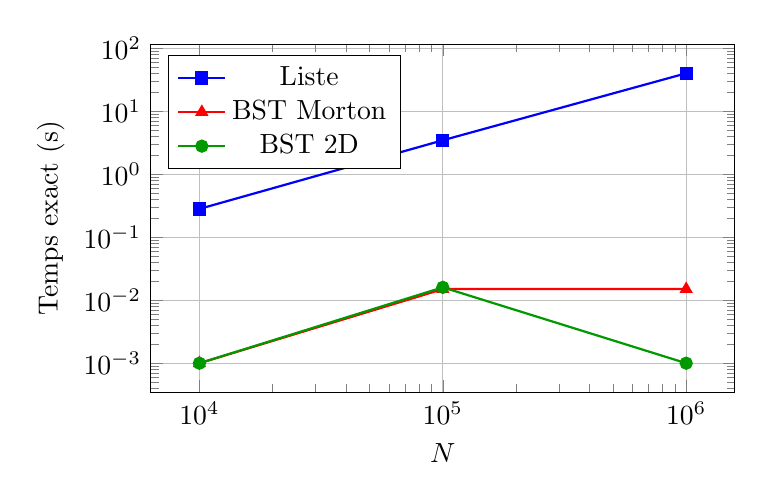
\begin{tikzpicture}
\begin{loglogaxis}[
    xlabel={$N$},
    ylabel={Temps exact (s)},
    legend pos=north west,
    xtick={10000,100000,1000000},
    xticklabels={$10^4$, $10^5$, $10^6$},
    width=9cm, height=6cm,
    grid=major
]
\addplot[blue, thick, mark=square*]
    coordinates {(10000,0.281)(100000,3.453)(1000000,39.936)};
\addlegendentry{Liste}
\addplot[red, thick, mark=triangle*]
    coordinates {(10000,0.001)(100000,0.015)(1000000,0.015)};
\addlegendentry{BST Morton}
\addplot[green!60!black, thick, mark=*]
    coordinates {(10000,0.001)(100000,0.016)(1000000,0.001)};
\addlegendentry{BST 2D}
\end{loglogaxis}
\end{tikzpicture}
\caption{Temps de recherche exacte en fonction de $N$ ($10^4$ requêtes positives)}
\end{figure}

\begin{figure}[H]
\centering
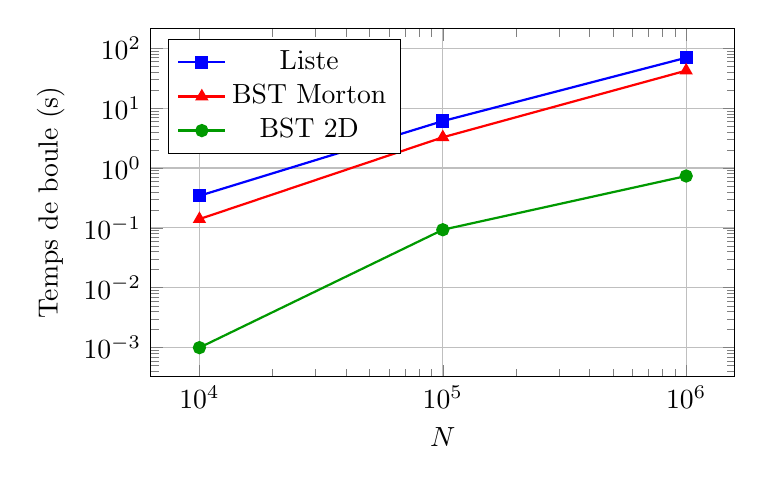
\begin{tikzpicture}
\begin{loglogaxis}[
    xlabel={$N$},
    ylabel={Temps de boule (s)},
    legend pos=north west,
    xtick={10000,100000,1000000},
    xticklabels={$10^4$, $10^5$, $10^6$},
    width=9cm, height=6cm,
    grid=major
]
\addplot[blue, thick, mark=square*]
    coordinates {(10000,0.343)(100000,6.062)(1000000,69.234)};
\addlegendentry{Liste}
\addplot[red, thick, mark=triangle*]
    coordinates {(10000,0.140)(100000,3.250)(1000000,42.173)};
\addlegendentry{BST Morton}
\addplot[green!60!black, thick, mark=*]
    coordinates {(10000,0.001)(100000,0.093)(1000000,0.734)};
\addlegendentry{BST 2D}
\end{loglogaxis}
\end{tikzpicture}
\caption{Temps de recherche en boule en fonction de $N$ ($r=0{,}01$, $10^4$ requêtes)}
\end{figure}

\subsection*{Variation du rayon ($N = 10^5$)}

\begin{center}
\begin{tabular}{lrrrr}
\toprule
$r$ & Résultats moy. & Liste & BST Morton & BST 2D \\
\midrule
0,01 & 31{,}1  & 6{,}06 s & 3{,}25 s  & \textbf{0{,}093 s} \\
0,05 & 751{,}7 & 6{,}00 s & 21{,}3 s  & \textbf{1{,}52 s}  \\
0,10 & 2876    & 7{,}72 s & 39{,}3 s  & \textbf{5{,}20 s}  \\
\bottomrule
\end{tabular}
\end{center}

\begin{figure}[H]
\centering
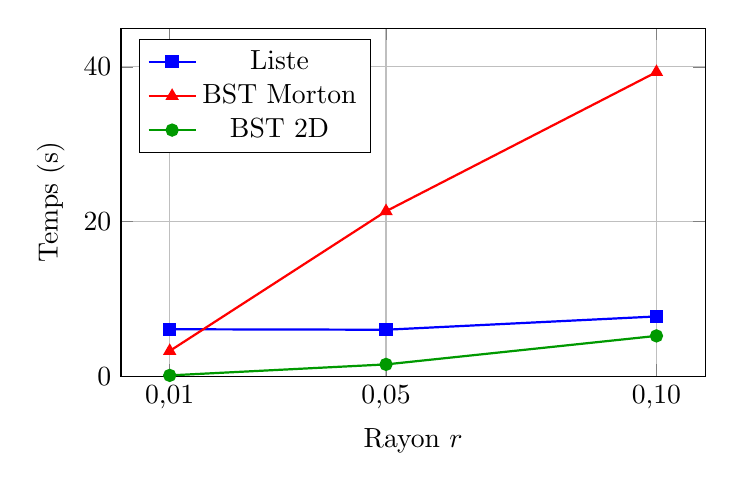
\begin{tikzpicture}
\begin{axis}[
    xlabel={Rayon $r$},
    ylabel={Temps (s)},
    legend pos=north west,
    xtick={0.01,0.05,0.1},
    xticklabels={0{,}01, 0{,}05, 0{,}10},
    ymin=0, ymax=45,
    width=9cm, height=6cm,
    grid=major
]
\addplot[blue, thick, mark=square*]
    coordinates {(0.01,6.062)(0.05,6.000)(0.1,7.718)};
\addlegendentry{Liste}
\addplot[red, thick, mark=triangle*]
    coordinates {(0.01,3.250)(0.05,21.327)(0.1,39.328)};
\addlegendentry{BST Morton}
\addplot[green!60!black, thick, mark=*]
    coordinates {(0.01,0.093)(0.05,1.516)(0.1,5.203)};
\addlegendentry{BST 2D}
\end{axis}
\end{tikzpicture}
\caption{Temps de recherche en boule en fonction du rayon ($N=10^5$, $10^4$ requêtes)}
\end{figure}
